\documentclass[12pt,twoside]{article}
\usepackage[dvipsnames]{xcolor}
\usepackage{tikz,graphicx,amsmath,amsfonts,amscd,amssymb,bm,cite,epsfig,epsf,url}
\usepackage[hang,flushmargin]{footmisc}
\usepackage[colorlinks=true,urlcolor=blue,citecolor=blue]{hyperref}
\usepackage{amsthm,multirow,wasysym,appendix}
\usepackage{array,subcaption} 
% \usepackage[small,bf]{caption}
\usepackage{bbm}
\usepackage{pgfplots}
\usetikzlibrary{spy}

\usepgfplotslibrary{external}
\usepgfplotslibrary{fillbetween}
\usetikzlibrary{arrows,automata}
\usepackage{thmtools}
\usepackage{blkarray} 
\usepackage{textcomp}
\usepackage[left=0.8in,right=1.0in,top=1.0in,bottom=1.0in]{geometry}

%% Probability operators and functions
%
% \def \P{\mathrm{P}}
\def \P{\mathrm{P}}
\def \E{\mathrm{E}}
\def \Var{\mathrm{Var}}
\let\var\Var
\def \Cov {\mathrm{Cov}} \let\cov\Cov
\def \MSE {\mathrm{MSE}} \let\mse\MSE
\def \sgn {\mathrm{sgn}}
\def \R {\mathbb{R}}
\def \C {\mathbb{C}}
\def \N {\mathbb{N}}
\def \Z {\mathbb{Z}}
\def \cV {\mathcal{V}}
\def \cS {\mathcal{S}}

\newcommand{\RR}{\ensuremath{\mathbb{R}}}

\DeclareMathOperator*{\argmin}{arg\,min}
\DeclareMathOperator*{\argmax}{arg\,max}
\newcommand{\red}[1]{\textcolor{red}{#1}}
\newcommand{\blue}[1]{\textcolor{blue}{#1}}
\newcommand{\green}[1]{\textcolor{ForestGreen}{ #1}}
\newcommand{\fuchsia}[1]{\textcolor{RoyalPurple}{ #1}}

\newcommand{\wrnd}[1]{\widetilde{ #1 } }
\newcommand{\po}{\wrnd{\op{po}}  }

%
%% Probability distributions
%
%\def \Bern    {\mathrm{Bern}}
%\def \Binom   {\mathrm{Binom}}
%\def \Exp     {\mathrm{Exp}}
%\def \Geom    {\mathrm{Geom}}
% \def \Norm    {\mathcal{N}}
%\def \Poisson {\mathrm{Poisson}}
%\def \Unif    {\mathrm {U}}
%
\DeclareMathOperator{\Norm}{\mathcal{N}}

\newcommand{\bdb}[1]{\textcolor{red}{#1}}

\newcommand{\ml}[1]{\mathcal{ #1 } }
\newcommand{\wh}[1]{\widehat{ #1 } }
\newcommand{\wt}[1]{\widetilde{ #1 } }
\newcommand{\conj}[1]{\overline{ #1 } }
\newcommand{\rnd}[1]{\tilde{ #1 } }
\newcommand{\rv}[1]{ \rnd{ #1}  }
\newcommand{\rM}{\rnd{ m}  }
\newcommand{\rx}{\rnd{ x}  }
\newcommand{\ry}{\rnd{ y}  }
\newcommand{\rz}{\rnd{ z}  }
\newcommand{\ra}{\rnd{ a}  }
\newcommand{\rb}{\rnd{ b}  }
\newcommand{\rt}{\rnd{ t}  }
\newcommand{\rs}{\rnd{ s}  }


\newcommand{\rpc}{\widetilde{ pc}  }
\newcommand{\rndvec}[1]{\vec{\rnd{#1}}}

\def \cnd {\, | \,}
\def \Id { I }
\def \J {\mathbf{1}\mathbf{1}^T}

\newcommand{\op}[1]{\operatorname{#1}}
\newcommand{\setdef}[2]{ := \keys{ #1 \; | \; #2 } }
\newcommand{\set}[2]{ \keys{ #1 \; | \; #2 } }
\newcommand{\sign}[1]{\op{sign}\left( #1 \right) }
\newcommand{\trace}[1]{\op{tr}\left( #1 \right) }
\newcommand{\tr}[1]{\op{tr}\left( #1 \right) }
\newcommand{\inv}[1]{\left( #1 \right)^{-1} }
\newcommand{\abs}[1]{\left| #1 \right|}
\newcommand{\sabs}[1]{| #1 |}
\newcommand{\keys}[1]{\left\{ #1 \right\}}
\newcommand{\sqbr}[1]{\left[ #1 \right]}
\newcommand{\sbrac}[1]{ ( #1 ) }
\newcommand{\brac}[1]{\left( #1 \right) }
\newcommand{\bbrac}[1]{\big( #1 \big) }
\newcommand{\Bbrac}[1]{\Big( #1 \Big)}
\newcommand{\BBbrac}[1]{\BIG( #1 \Big)}
\newcommand{\MAT}[1]{\begin{bmatrix} #1 \end{bmatrix}}
\newcommand{\sMAT}[1]{\left(\begin{smallmatrix} #1 \end{smallmatrix}\right)}
\newcommand{\sMATn}[1]{\begin{smallmatrix} #1 \end{smallmatrix}}
\newcommand{\PROD}[2]{\left \langle #1, #2\right \rangle}
\newcommand{\PRODs}[2]{\langle #1, #2 \rangle}
\newcommand{\der}[2]{\frac{\text{d}#2}{\text{d}#1}}
\newcommand{\pder}[2]{\frac{\partial#2}{\partial#1}}
\newcommand{\derTwo}[2]{\frac{\text{d}^2#2}{\text{d}#1^2}}
\newcommand{\ceil}[1]{\lceil #1 \rceil}
\newcommand{\Imag}[1]{\op{Im}\brac{ #1 }}
\newcommand{\Real}[1]{\op{Re}\brac{ #1 }}
\newcommand{\norm}[1]{\left|\left| #1 \right|\right| }
\newcommand{\norms}[1]{ \| #1 \|  }
\newcommand{\normProd}[1]{\left|\left| #1 \right|\right| _{\PROD{\cdot}{\cdot}} }
\newcommand{\normTwo}[1]{\left|\left| #1 \right|\right| _{2} }
\newcommand{\normTwos}[1]{ \| #1  \| _{2} }
\newcommand{\normZero}[1]{\left|\left| #1 \right|\right| _{0} }
\newcommand{\normTV}[1]{\left|\left| #1 \right|\right|  _{ \op{TV}  } }% _{\op{c} \ell_1} }
\newcommand{\normOne}[1]{\left|\left| #1 \right|\right| _{1} }
\newcommand{\normOnes}[1]{\| #1 \| _{1} }
\newcommand{\normOneTwo}[1]{\left|\left| #1 \right|\right| _{1,2} }
\newcommand{\normF}[1]{\left|\left| #1 \right|\right| _{\op{F}} }
\newcommand{\normLTwo}[1]{\left|\left| #1 \right|\right| _{\ml{L}_2} }
\newcommand{\normNuc}[1]{\left|\left| #1 \right|\right| _{\ast} }
\newcommand{\normOp}[1]{\left|\left| #1 \right|\right|  }
\newcommand{\normInf}[1]{\left|\left| #1 \right|\right| _{\infty}  }
\newcommand{\proj}[1]{\mathcal{P}_{#1} \, }
\newcommand{\diff}[1]{ \, \text{d}#1 }
\newcommand{\vc}[1]{\boldsymbol{\vec{#1}}}
\newcommand{\rc}[1]{\boldsymbol{#1}}
\newcommand{\vx}{\vec{x}}
\newcommand{\vy}{\vec{y}}
\newcommand{\vz}{\vec{z}}
\newcommand{\vu}{\vec{u}}
\newcommand{\vv}{\vec{v}}
\newcommand{\vb}{\vec{\beta}}
\newcommand{\va}{\vec{\alpha}}
\newcommand{\vaa}{\vec{a}}
\newcommand{\vbb}{\vec{b}}
\newcommand{\vg}{\vec{g}}
\newcommand{\vw}{\vec{w}}
\newcommand{\vh}{\vec{h}}
\newcommand{\vbeta}{\vec{\beta}}
\newcommand{\valpha}{\vec{\alpha}}
\newcommand{\vgamma}{\vec{\gamma}}
\newcommand{\veta}{\vec{\eta}}
\newcommand{\vnu}{\vec{\nu}}
\newcommand{\rw}{\rnd{w}}
\newcommand{\rvnu}{\vc{\nu}}
\newcommand{\rvv}{\rndvec{v}}
\newcommand{\rvw}{\rndvec{w}}
\newcommand{\rvx}{\rndvec{x}}
\newcommand{\rvy}{\rndvec{y}}
\newcommand{\rvz}{\rndvec{z}}
\newcommand{\rvX}{\rndvec{X}}


\newtheorem{theorem}{Theorem}[section]
% \declaretheorem[style=plain,qed=$\square$]{theorem}
\newtheorem{corollary}[theorem]{Corollary}
\newtheorem{definition}[theorem]{Definition}
\newtheorem{lemma}[theorem]{Lemma}
\newtheorem{remark}[theorem]{Remark}
\newtheorem{algorithm}[theorem]{Algorithm}

% \theoremstyle{definition}
%\newtheorem{example}[proof]{Example}
\declaretheorem[style=definition,qed=$\triangle$,sibling=definition]{example}
\declaretheorem[style=definition,qed=$\bigcirc$,sibling=definition]{application}

%
%% Typographic tweaks and miscellaneous
%\newcommand{\sfrac}[2]{\mbox{\small$\displaystyle\frac{#1}{#2}$}}
%\newcommand{\suchthat}{\kern0.1em{:}\kern0.3em}
%\newcommand{\qqquad}{\kern3em}
%\newcommand{\cond}{\,|\,}
%\def\Matlab{\textsc{Matlab}}
%\newcommand{\displayskip}[1]{\abovedisplayskip #1\belowdisplayskip #1}
%\newcommand{\term}[1]{\emph{#1}}
%\renewcommand{\implies}{\;\Rightarrow\;}



\newcommand{\ru}{\rnd{ u}  }
\newcommand{\rd}{\rnd{ d}  }
%\newcommand{\rs}{\rnd{ s}  }
\newcommand{\ri}{\rnd{ i}  }
\newcommand{\re}{\rnd{ e}  }
\newcommand{\rQ}{\rnd{ q}  }
\newcommand{\rC}{\rnd{ c}  }


\begin{document}

\begin{center}
{\large{\textbf{Homework 10}} } \vspace{0.2cm}\\
Due  at 11 pm
\\
\end{center}
Unless stated otherwise, justify any answers you give.
You can work in groups, but each
student must write their own solution based on their own
understanding of the problem.

When uploading your homework to Gradescope you will have to
select the relevant pages for each question.  Please submit each
problem on a separate page (i.e., 1a and~1b can be on the same page but 1
and 2 must be on different pages).  We understand that this may be
cumbersome but this is the best way for the grading team to grade your
homework assignments and provide feedback in a timely manner.  Failure
to adhere to these guidelines may result in a loss of points.
Note that it may take some time to
select the pages for your submission.  Please plan accordingly.  We
suggest uploading your assignment at least 30 minutes before the deadline
so you will have ample time to select the correct pages for your
submission.  If you are using \LaTeX, consider using the minted or
listings packages for typesetting code.  
\\

\begin{enumerate}

\item (Life expectancy) During the Middle Ages, life expectancy was much shorter than in modern times. According to some calculations the mean age of death was 37.5 years. To some extent, this was driven by the high infant mortality: %The probability of dying by the age of 4 was as high as 0.4 during the Middle Ages. Right now in the United States it is negligible by comparison (around 0.007). 
it has been estimated that the probability of dying during the first year of age was 0.25. If we assign an age of death equal to zero to anyone dying in their first year, what was the mean age of death of the people who survived the first year? 

\begin{itemize}
    \item note that we can express $E[\tilde{a}|\tilde{a}>0]=\Sigma_{i=1}^{\infty}ap_{a|a>0}(a|a>0)=\Sigma_{i=1}^{\infty}a\frac{p_{a}(a)}{P(a>0)}=\frac{1}{P(a>0)}\Sigma+{i=1}^{\infty}ap_{a}(a)+0*P_{a}(a)=\frac{1}{P(a>0)}\Sigma+{i=1}^{\infty}ap_{a}(a)=\frac{E(a)}{P(a>0)}=\frac{E(a)}{1-P(a<0)}=\frac{E(a)}{1-P_{a}(0)}=\frac{37.5}{1-.25}=50$
    
\end{itemize}

\item (Law of conditional variance) 
We define the conditional variance function $\nu_{\rb \cnd \ra}(a)$ of a random variable $\rb$ given another random variable $\ra$ as the variance of $\rb$ conditioned on the event $\ra = a$. Analogously to the conditional mean, we define the conditional variance $\nu_{\rb \cnd \ra}(\ra)$ of $\rb$ given $\ra$ as the random variable obtained by plugging $\ra$ into the conditional variance function. 
\begin{enumerate}
\item Compute the conditional variance function $\nu_{\rb \cnd \ra}$ for the random variables $\ra$ and $\rb$ in Example 7.45.
\begin{itemize}
\item we can find $v_{\Tilde{b}|\Tilde{a}}(a)=\Sigma_{b=0}^{3}b^2P(b|a)-(\Sigma_{b=0}^{3}b^2P(b|a))^2$
\item this yields $v_{\Tilde{b}|\Tilde{a}}(1)=\frac{20}{49}$,$v_{\Tilde{b}|\Tilde{a}}(2)=\frac{38}{49}$, $v_{\Tilde{b}|\Tilde{a}}(3)=\frac{2}{3}$
\end{itemize}
\item Compute the pmf of the conditional variance $\nu_{\rb \cnd \ra}(\ra)$ for the random variables $\ra$ and $\rb$ in Example 7.45. 
\begin{itemize}
    \item we know that $v_{\Tilde{b}|\Tilde{a}}(a)$ is a deterministic function, so plugging in the random variable $\Tilde{a}$ yields us the random variable $v_{\Tilde{b}|\Tilde{a}}(\Tilde{a})$ whose pmf is completely determined by $\Tilde{a}$. that is $P_{v_{\Tilde{b}|\Tilde{a}}(\Tilde{}{a})}(x)=P_{\Tilde{a}}(a)$
    \item thus we know that $P(v_{\Tilde{b}|\Tilde{a}}(a)=\frac{20}{49})=p(\Tilde{a}=1)=\frac{7}{20}$,\item $P(v_{\Tilde{b}|\Tilde{a}}(a)=\frac{38}{49})=p(\Tilde{a}=2)=\frac{7}{20} $\item
    $P(v_{\Tilde{b}|\Tilde{a}}(a)=\frac{2}{3})=p(\Tilde{a}=3)=\frac{7}{20}=\frac{6}{20} $
\end{itemize}
\item Prove the law of conditional variance:
\begin{align}
\Var( \ssqbr{\rb} )= \E \sqbr{ \nu_{\rb \cnd \ra}(\ra) } + \Var \sqbr{ \mu_{\rb \cnd \ra}(\ra) }.
\end{align}
\begin{itemize}
    \item we can express $Var(\mu_{\Tilde{b}|\Tilde{a}}(\Tilde{a}))$ as $E[\mu_{\Tilde{b}|\Tilde{a}}(\Tilde{a})^2]-E[\mu_{\Tilde{b}|\Tilde{a}}(\Tilde{a})]^2$ by the law of iterated expectations we can write $E[\mu_{\Tilde{b}|\Tilde{a}}(\Tilde{a})]=E[\Tilde{b}]$ thus we have $Var(\mu_{\Tilde{b}|\Tilde{a}}(\Tilde{a}))=E[\mu_{\Tilde{b}|\Tilde{a}}(\Tilde{a})^2]-E[\Tilde{b}]^2$
    \item looking at$E[v_{\Tilde{b}|\Tilde{a}}(\Tilde{a})]$ we know that $v_{\Tilde{b}|\Tilde{a}}(\Tilde{a})=E[\tilde{b}^2|\tilde{a}]-E[\tilde{b}|\tilde{a}]^2=\Sigma_{b\in B}b^2*P_{\tilde{b}|\tilde{a}}(b|a)-(\Sigma_{b\in B}b*P_{\tilde{b}|\tilde{a}}(b|a))^2=\mu_{\tilde{b}^2|\tilde{a}}(\tilde{a})-\mu_{\tilde{b}|\tilde{a}}(\tilde{a})^2$
    \item thus we can see that $E[v_{\Tilde{b}|\Tilde{a}}(\Tilde{a})]=E[\mu_{\tilde{b}^2|\tilde{a}}(\tilde{a})-\mu_{\tilde{b}|\tilde{a}}(\tilde{a})^2]=E[\mu_{\tilde{b}^2|\tilde{a}}(\tilde{a})]-E[\mu_{\tilde{b}|\tilde{a}}(\tilde{a})^2]=E[\tilde{b}^2]-E[\mu_{\tilde{b}|\tilde{a}}(\tilde{a})^2]$
    \item putting these two things terms together we have $ \E \sqbr{ \nu_{\rb \cnd \ra}(\ra) } + \Var \sqbr{ \mu_{\rb \cnd \ra}(\ra) }=E[\tilde{b}^2]-E[\mu_{\Tilde{b}|\Tilde{a}}(\Tilde{a})^2]+E[\mu_{\Tilde{b}|\Tilde{a}}(\Tilde{a})^2]-E[\Tilde{b}]^2=E[\tilde{b}^2]-E[\Tilde{b}]^2=var(\tilde{b})$ proving the identity
\end{itemize}
\item Verify that the law of conditional variance holds for the random variables $\ra$ and $\rb$ in Example 7.45. 
\begin{itemize}
   \item $\mu_{b}=2.15$
   \item $var(\tilde{b})=.625$
   \item $E[v_{b|a}(a)]=6.145$
   \item $\mu_{\mu_{b|a}}(a)=\mu_{b}=2.15$
   \item $var(\mu_{b|a}(a)=.0127$
   \item $E[v_{b|a}(a)]+var(\mu_{b|a}(a)=.62$
   \item so the equality approximately holds
\end{itemize}
\end{enumerate}

\item (Weight-loss supplement) In order to evaluate the effectiveness of a weight-loss supplement, we record the weight gain/loss in kilograms after one month of a treatment group that takes the supplement, and a control group that doesn't. In bold, we highlight the participants who reported that they exercise daily.

Supplement: 0.5, \textbf{-4.6}, \textbf{-7.5}, 1.1, \textbf{-3.4}, \textbf{-1.4}, \textbf{3.2}, -1.9, \textbf{-3.6}, 2.4, 1.2, \textbf{4.2}, \textbf{-2.5}, \textbf{-3.5}, 4.7 \\ 
No supplement: 1.6, \textbf{-6.7}, 2.3, \textbf{-4.5}, \textbf{3.4}, -0.6, 2.3, 1.5, 1.7,2.6, 0.5, 1.2, \textbf{-3.6}, 2.1, -1.2, 0.4
\begin{enumerate}
\item Compute the unadjusted average treatment effect (ATE) given by the difference in average weight gain/loss between the treatment and control groups. 
\begin{itemize}
    \item  we can compute the unadjusted ATE as $E[\tilde{po_{1}}]-E[\tilde{po_{0}}]=\Sigma_{p\in po_1}p*P_{\tilde{po_{1}}}(p)-\Sigma_{p\in po_0}p*P_{\tilde{po_{0}}}(p)=-.74-(.1875)=-.92$
\end{itemize}

\item Estimate the ATE making any adjustments that you think are reasonable. Explain under what assumptions your estimate approximates the true ATE. 
\begin{itemize}
    \item let us assume that potential outcomes are conditionally independent given if a person works out every day or not (which we can call $\tilde{c}$)
    \item this assumption allows us to adjust our training data for this potential confounder that is we can write adjusted ate= $E[\tilde{po_{1}}]-E[\tilde{po_{0}}]=\Sigma_{c=0}^{1}\mu_{po_1|c}P_{\tilde{c}(c)}-\Sigma_{c=0}^{1}\mu_{po_0|c}P_{\tilde{c}(c)}=\Sigma_{c=0}^{1}(\Sigma_{p\in po_1}pP_{po_1}(p))P_{\tilde{c}(c)}-\Sigma_{c=0}^{1}(\Sigma_{p\in po_0}pP_{po_0}(p))P_{\tilde{c}(c)}=\frac{13}{31}(-2.12)+\frac{18}{31}1.33-\frac{13}{31}(-2.85)-\frac{18}{31}1.2=0.38161$
    \item thus controlling for the confounder of if a person exercised every day we can see that the ATE of the supplement is about -1 point 
\end{itemize}

\end{enumerate}


\item (Shared bike rides and temperature) 
In this question, we use \href{https://ride.capitalbikeshare.com/system-data}{share bike data} to study the relationship between daily number of rides and temperature. We perform our analysis on a cleaned and subsampled version of the data, \texttt{day.csv}. Complete \texttt{bike.ipynb} and answer the following questions.
\begin{enumerate}
\item Plot an estimate of the conditional mean of daily ride count given the temperature along with the scatter plot of data. Justify any choices you make.
\begin{itemize}
    \item we are assuming that there is some function $f(w,x)$ with learned weights that can approximate y in such a way that $y=f(x,w)+\epsilon$ where $\epsilon\sim \mathcal{N}(0,\sigma^2) $ that is we are assuming there is a function that can get x to approximate y in a way that its error is normally distributed with mean 0. once we have made this assumption it is justified to sellect f(x) such that $f(x)=argmin_{f(x)}\Sigma_{i=1}^{n}(f(x_i)-y_i)^2$ is 
    \item 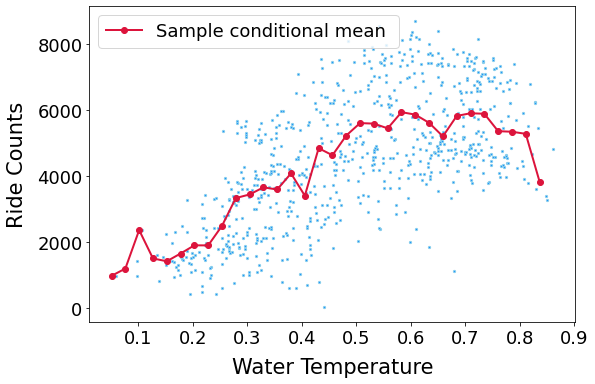
\includegraphics[width=10cm]{homework 10/CHART_2.png}
\end{itemize}
\item Annotate your plot to incorporate the conditional standard deviation of daily ride count given the temperature (apart from plotting the conditional mean, plot the conditional mean $\pm$ the conditional standard deviation).
\item 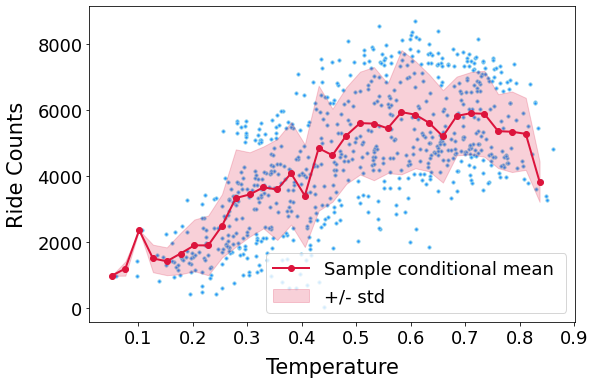
\includegraphics[width=10cm]{homework 10/CHART_1.png}
\item Do you expect your estimates to be equally reliable at every point? Please explain your reasoning. (We are not looking for a mathematical answer, you can just explain intuitively.)

\begin{itemize}
    \item we are fitting a parametric model to the data, so at points where there is less data, I would expect our model to over fit more, and thus be less reliable. 
    
\end{itemize}

\end{enumerate}


\end{enumerate}
\end{document}
